%--------------------------
% CHAPTER 5: Specification
%--------------------------

\chapter{Specification}

\label{chapter05}

As explained before, the \thesis\ is a big data problem, but in order to this amount of data be useful and make actual sense, the data model must be correct and very well defined. If there is some conceptual mistake the data displayed in the charts will not be reliable, so it will not be satisfying non-functional requirement of reliability (\#5).
\\\\
The data model must be also subject to change and pretty clear, to fulfill non-functional requirement of Maintainability (\#7).

%-----------------
%   SECTION 5.1
%-----------------

\section{Routes model} \label{routes_model}

\squad's pipeline, writes the data in \textbf{Single Flight Number} model. This model is not useful for this project because of the \nameref{sfn-date-set} schema. The timetable pipeline can also write following the \textbf{unified timetable} schema, this model presents the final master set of single flight number timetables that have been merged and de-duplicated from multiple sources. Dates schema are compatible with the \thesis\ purpose.

\subsection{Single Flight Number Object Model} \label{sfn-model}

The \textbf{Single Flight Number} (SFN) timetables data schema is designed with the following object model.

\subsubsection*{SFN Route}

Represents a route between 2 airports and the SFNs timetable that are available on that route. It is composed by three fields:

\begin{table}[H]
\centering
\begin{tabular}{|>{\raggedright\arraybackslash}p{2.5cm}|>{\raggedright\arraybackslash}p{4cm}|>{\raggedright\arraybackslash}p{2.5cm}|>{\raggedright\arraybackslash}p{2cm}|>{\raggedright\arraybackslash}p{1.2cm}|}
\hline
\textbf{Field}       & \textbf{Description}                                 & \textbf{Data Type}           & \textbf{Required} & \textbf{Key} \\ \hline
\textbf{Origin}      & The origin airport or station for the timetable      & Integer                      & Yes               & Yes          \\ \hline
\textbf{Destination} & The destination airport or station for the timetable & Integer                      & Yes               & Yes          \\ \hline
\textbf{Series}      & The SFN timetables associated with the route         & List of SFN Timetable Series & Yes               & No           \\ \hline
\end{tabular}
\caption{Single Flight Number Route fields}
\label{sfn-route}
\end{table}

\subsubsection*{SFN Timetable Series}

Represents a SFN timetable for the year ahead.

\begin{table}[H]
\centering
\begin{tabular}{|>{\raggedright\arraybackslash}p{2.5cm}|>{\raggedright\arraybackslash}p{4cm}|>{\raggedright\arraybackslash}p{2.5cm}|>{\raggedright\arraybackslash}p{2cm}|>{\raggedright\arraybackslash}p{1.2cm}|}
\hline
\textbf{Field}                           & \textbf{Description}                               & \textbf{Data Type}      & \textbf{Required} & \textbf{Key} \\ \hline
\textbf{Marketing Carrier}               & The ID of the carrier that is marketing the flight & Integer                 & Yes               & Yes          \\ \hline
\textbf{Marketing Carrier Flight Number} & The flight code assigned by the marketing carrier  & Integer                 & Yes               & Yes          \\ \hline
\textbf{Series Items}                    & 1..n Series Items                                  & List of SFN Series Item & Yes               & No           \\ \hline
\end{tabular}
\caption{Single Flight Number Timetable Series fields}
\label{sfn-series}
\end{table}

\subsubsection*{SFN Timetable Series Item}

A Timetable Series Item represents a specific configurations of operating carrier, stops and times of day for a given SFN timetable. For example for a given Marketing Carrier / Flight Number, the Operating Carrier or times of day may change through the year.

\begin{table}[H]
\centering
\begin{tabular}{|>{\raggedright\arraybackslash}p{2.5cm}|>{\raggedright\arraybackslash}p{4cm}|>{\raggedright\arraybackslash}p{2.5cm}|>{\raggedright\arraybackslash}p{2cm}|>{\raggedright\arraybackslash}p{1.2cm}|}
\hline
\textbf{Field}                           & \textbf{Description}                                                                           & \textbf{Data Type}            & \textbf{Required} & \textbf{Key} \\ \hline
\textbf{Operating Carrier}               & The ID of the administrating operating Carrier                                                 & Integer                       & Yes               & Yes          \\ \hline
\textbf{Operating Carrier Flight Number} & The flight code assigned by the administrating operating carrier                               & Integer                       & No                & No           \\ \hline
\textbf{Physical Operating Carrier}      & The ID of the 'physical' operating Carrier                                                     & Integer                       & Yes               & Yes          \\ \hline
\textbf{Stop Count}                      & The total number of stops (can be derived from the list of stops)                              & Integer                       & Yes               & No           \\ \hline
\textbf{Stops}                           & A list of via airports                                                                         & List of Integer               & No                & Yes          \\ \hline
\textbf{Departure time}                  & The time of departure in the current time zone of the origin station (minutes after 00:00)     & Integer                       & Yes               & Yes          \\ \hline
\textbf{Arrival time}                    & The time of arrival in the current time zone of the destination station (minutes after 00:00)  & Integer                       & Yes               & Yes          \\ \hline
\textbf{Arrival day offset}              & The number of days after the departure date that the flight arrives                            & Integer                       & Yes               & Yes          \\ \hline
\textbf{Duration}                        & The total flight duration (can be derived from the departure and arrival times and day offset) & Integer                       & Yes               & No           \\ \hline
\textbf{Traffic Restrictions}            & Restrictions relating to how a flight can be sold                                              & Traffic Restrictions instance & Yes               & Yes          \\ \hline
\textbf{DateSets}                        & The dates that this Timetable Series Item is flown                                             & Array of DateSet              & Yes               & No           \\ \hline
\end{tabular}
\caption{Single Flight Number Timetable Series Item fields}
\label{sfn-series-item}
\end{table}

\subsubsection*{Traffic restrictions}

A set of flags indicating restrictions relating to how an timetabled flight might be sold. Not relevant for this project.

\subsubsection*{SFN Date Set} \label{sfn-date-set}

A Date Set represents a start date and day of week pattern for a given Timetable Series Item.

\begin{table}[H]
\centering
\begin{tabular}{|>{\raggedright\arraybackslash}p{2.5cm}|>{\raggedright\arraybackslash}p{4.7cm}|>{\raggedright\arraybackslash}p{3cm}|>{\raggedright\arraybackslash}p{2cm}|}
\hline
\textbf{Field}        & \textbf{Description}                                                                                  & \textbf{Data Type}              & \textbf{Required} \\ \hline
\textbf{Start Date}   & The start date that this set is applicable from                                                       & String (date format YYYY-MM-DD) & Yes               \\ \hline
\textbf{Data Sources} & The source(s) of the timetable data                                                                   & Array of sources (Enun)         & Yes               \\ \hline
\textbf{Availability} & A set of offsets indicating the dates that the associated series is available (up to 13 months ahead) & Array of week days (Enum)       & Yes               \\ \hline
\end{tabular}
\caption{Single Flight Number Timetable Date set fields}
\label{sfn-date-set}
\end{table}

Since the dates are represented by week days as an enumeration (\textit{mon}, \textit{tue}, \textit{wed}, ...), the grouping of flights by \textbf{day} or \textbf{month}\footnote{The model changes and the pipelines groups by month. Learn why here: \nameref{month_version} on page \pageref{month_version}} becomes very difficult and non trivial. That is why the \thesis\ uses the \textbf{Unified} model.

\subsection{Unified Timetable Object Model} \label{unified-model}

In the timetable pipeline owned by \squad\ first maps all data to Unified model then it is mapped to the final Single Flight Number Timetable model. Unified model is very similar than \nameref{sfn-model}, it uses \textbf{Airport object} instead of an integer and a set of strings in date format \texttt{YYYY-MM-DD} in date sets, availability:

\begin{figure}[H]
\centering
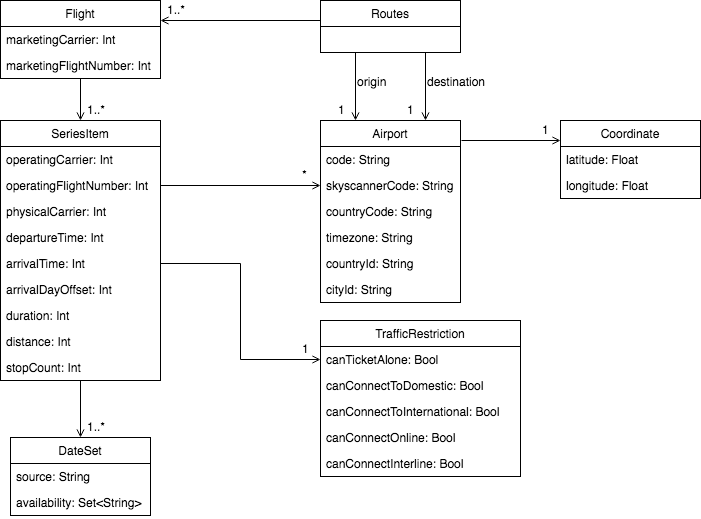
\includegraphics[scale=0.6]{diagrams/unified_model.png}
\caption{Unified Timetables UML class diagram}
\label{unified-uml}
\end{figure}

With this model, the \nameref{available-flights-pipeline} can apply flattening and grouping easily.
\\\\
Airport's code will be used to identify them and pairs of codes will represent a route. This code is also know as IATA Code\cite{iata_code}.

%-----------------
%   SECTION 5.2
%-----------------

\section{Searches model}

The user searches are stored in a huge database that contains flight search, car hire search and hotel search, one has value an the other two are \texttt{null}.

\begin{figure}[H]
\centering
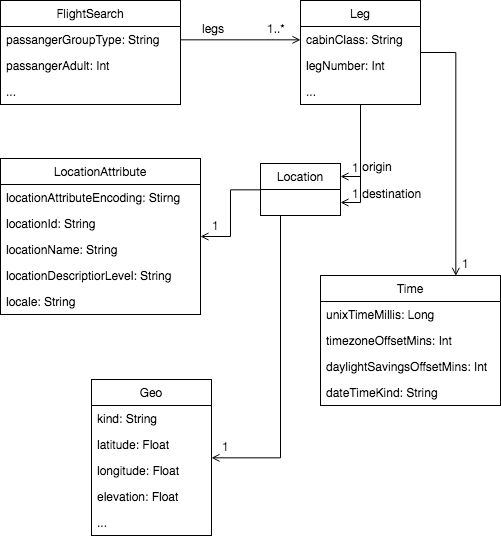
\includegraphics[scale=0.6]{diagrams/flight_search.png}
\caption{Flight search UML class diagram}
\end{figure}

A user query in \company\ contains a lot of information, but most of it is not useful for the purpose of this project.

%-----------------
%   SECTION 5.3
%-----------------

\section{Available Fligths Model} \label{flight-availablity-model}

As we can see above in the \nameref{unified-model}, flights are grouped by routes, then by flights, series and finally we reach the date. The \thesis\ will be queried by route and date, so it is important to have the flights stored and count its availability at date level.
\\\\
The flights availability records will be grouped by route and then by date.

\begin{figure}[H]
\centering
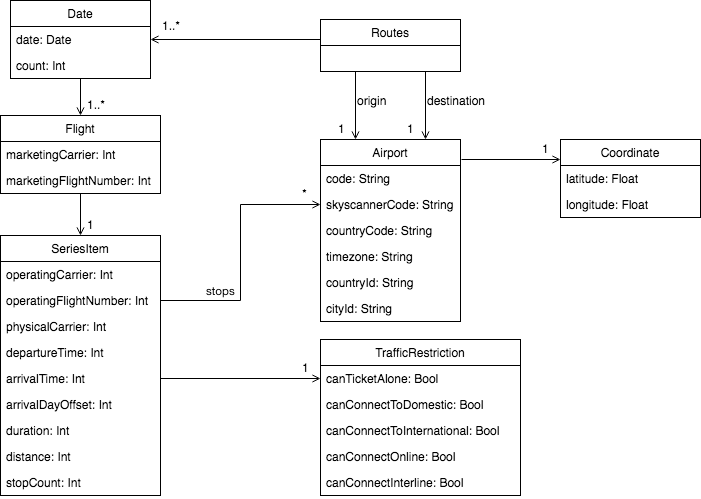
\includegraphics[scale=0.6]{diagrams/flights_availability_model.png}
\caption{Flights Availability UML class diagram}
\end{figure}

Flights Availability and \nameref{unified-uml} looks very similar. The main difference is that a route in Unified model contains a set of flights but a set of dates in Flight Availability.
\\\\
Date class contains a strings in date format \texttt{YYYY-MM-DD} and the number of available flights on that date. This last field is the same as the size of the set of flights it is composed by. The flight availability model has \textbf{a lot of duplicated values}, one flight operates a lot of dates and it is grouped by date\footnote{All flights data transformations explained in \nameref{fop-data-transformations}}.

%-----------------
%   SECTION 5.4
%-----------------

\section{User Searches Model}

The user searches model has been simplified and a lot of fields from the original model has been removed. Since the amount of data of user searches increases on the order of millions per day, the model contains the basic data.

\subsubsection*{User Searches Route}

\begin{table}[H]
\centering
\begin{tabular}{|>{\raggedright\arraybackslash}p{2.5cm}|>{\raggedright\arraybackslash}p{4cm}|>{\raggedright\arraybackslash}p{2.5cm}|>{\raggedright\arraybackslash}p{2cm}|>{\raggedright\arraybackslash}p{1.2cm}|}
\hline
\textbf{Field}       & \textbf{Description}                         & \textbf{Data Type}     & \textbf{Required} & \textbf{Key} \\ \hline
\textbf{Origin}      & The origin airport or station IATA code      & String                 & Yes               & Yes          \\ \hline
\textbf{Destination} & The destination airport or station IATA code & String                 & Yes               & Yes          \\ \hline
\textbf{Dates}       & The SFN timetables associated with the route & List of Searches Dates & Yes               & No           \\ \hline
\end{tabular}
\caption{User Searches Route fields}
\end{table}

\subsubsection*{Searches Date}

\begin{table}[H]
\centering
\begin{tabular}{|>{\raggedright\arraybackslash}p{2.5cm}|>{\raggedright\arraybackslash}p{4cm}|>{\raggedright\arraybackslash}p{2.5cm}|>{\raggedright\arraybackslash}p{2cm}|>{\raggedright\arraybackslash}p{1.2cm}|}
\hline
\textbf{Field} & \textbf{Description}                           & \textbf{Data Type} & \textbf{Required} & \textbf{Key} \\ \hline
\textbf{Date}  & Date for the leg that was searched             & String             & Yes               & Yes          \\ \hline
\textbf{Count} & Number of searches for that route in that date & Integer            & Yes               & No           \\ \hline
\end{tabular}
\caption{Searches Date fields}
\end{table}







